\chapter{Polarisation Spectroscopy}\label{chapter:pol_spec}

{\color{red}More discussion/intro to pol spec.

Lonely orphans from another section:

Pol Spec developments

It has been shown previously that \gls*{ps} can be used to reduce the linewidth of a distributed feedback diode from \unit[2]{MHz} to \unit[20]{kHz}~\cite{torii_laser-phase_2012} and of \glspl*{ecdl} to \unit[65]{kHz}
~\cite{yoshikawa_frequency_2003}.

Balanced polarimeter.\cite{pearman_polarization_2002,yoshikawa_frequency_2003}

Bi-polarisation spectroscopy.\cite{tiwari_laser_2006}

}

\section{Basic Theory}\label{section:pol_spec_theory}

In \gls{ps} a circularly polarised pump beam from a monochromatic laser, with frequency close to an atomic resonance, induces frequency-dependent circular birefringence in a magnetically-shielded atomic gas sample.
A linearly polarised beam from the same source is used to measure the birefringence, monitored with a balanced polarimeter consisting of a half-wave phase retarder, \gls{pbs} and two detectors.
This is shown in Figure \ref{figure:pol_spec_schematic}.

\begin{figure}
\centering
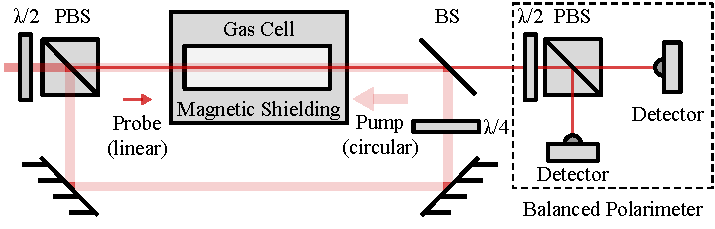
\includegraphics[width=\linewidth]{part1/Figs/PolSpecSchematic.pdf}
\caption{A schematic of \gls{ps} with a balanced polarimeter.
The power balance between the probe and the pump beam is controlled with the left-most $\lambda/2$ phase retarder and \gls{pbs}.
The $\lambda/4$ retarder is adjusted to produce a circularly polarised pump beam.
The non-polarising beamsplitter (BS) is used to counter-propagate the pump beam through the atomic sample without altering the polarisation of the circular pump or linear probe.
The final $\lambda/2$ retarder, \gls{pbs} and the detectors form the balanced polarimeter that monitors the polarisation rotation of the probe.}
\label{figure:pol_spec_schematic}
\end{figure}

The circularly polarised pump beam induces circular birefringence in the atomic sample by partially optically pumping the sample into one of the extreme hyperfine sublevels, $m_F=\pm F$, where $m_F$ labels the hyperfine sublevel and $F$ labels {\color{red}some quantum thingy.}
This partial optical pumping, referred to here as the anisotropy of the medium, results in unequal absorption coefficients for each circular polarisation.
The linearly polarised probe beam can be decomposed into two equal and oppositely circularly polarised components which undergo different absorption due to the anisotropy, such that when recombined after passing through the atomic sample the probe beam becomes elliptically polarised with an angle different to that of the original linear polarisation.
This process is depicted in Figure \ref{figure:pol_spec_explanation}.

\begin{figure}
\centering
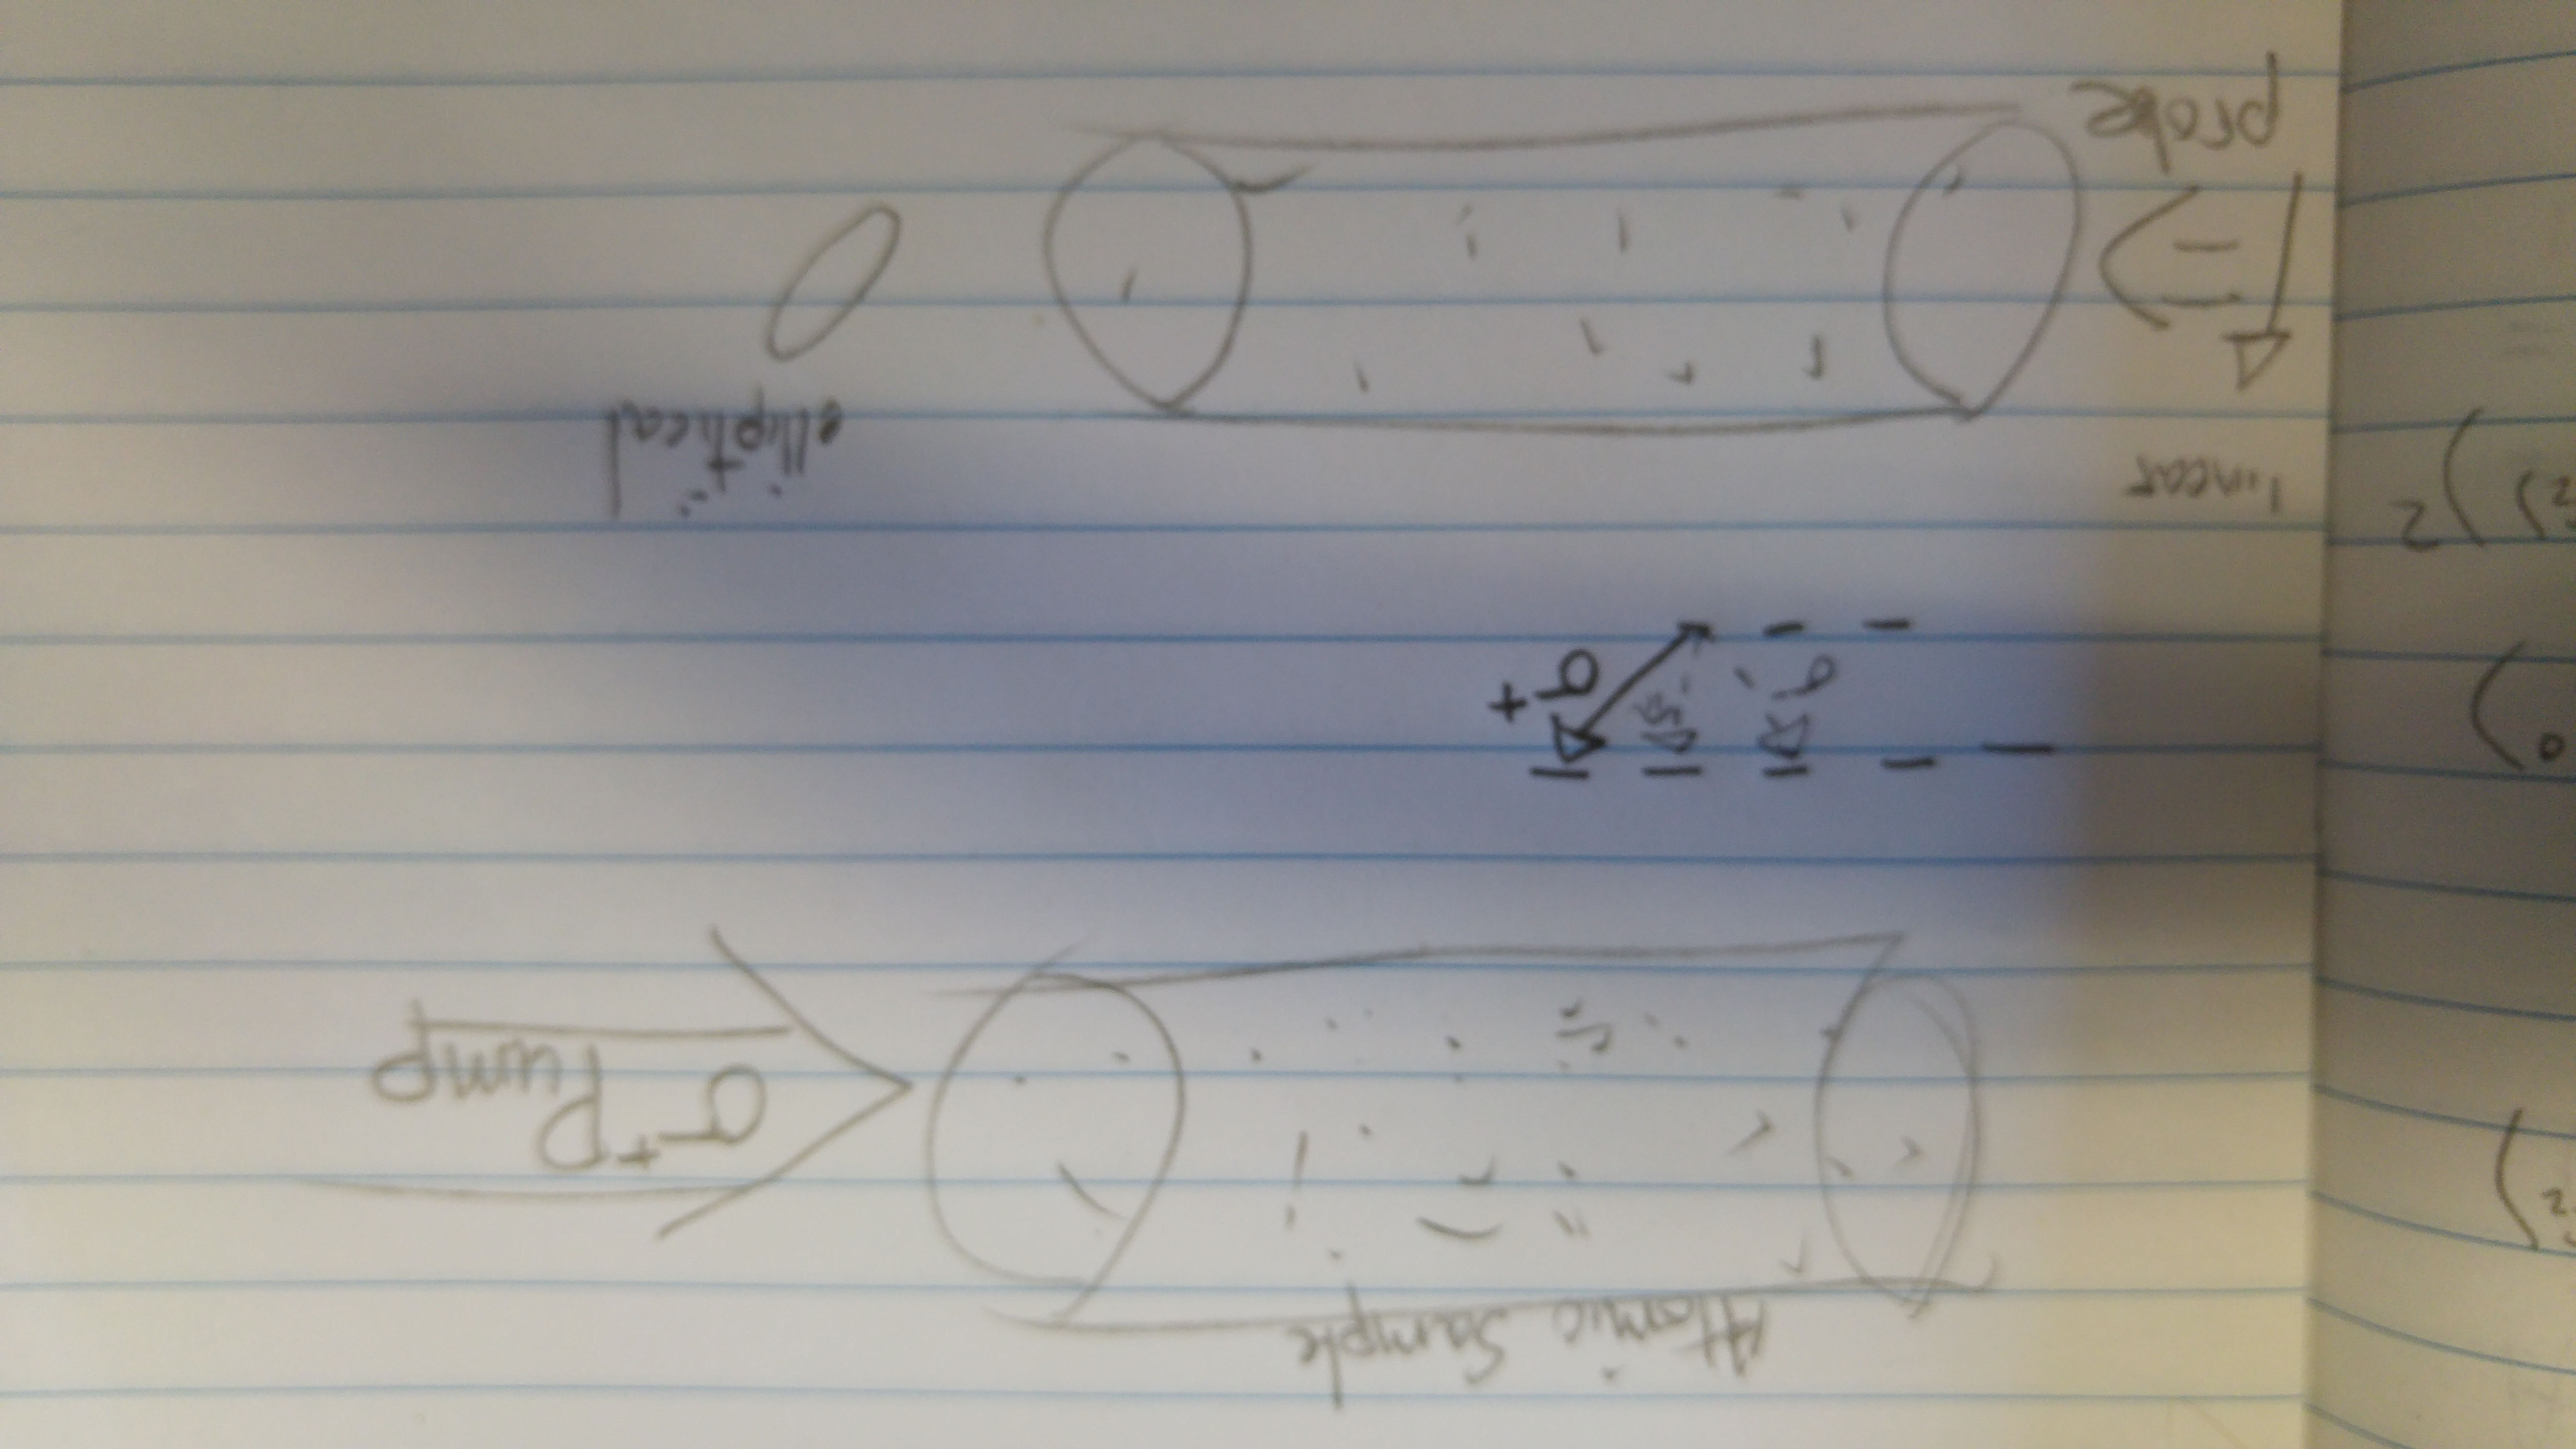
\includegraphics[width=\linewidth,angle=180]{part1/Figs/pol_spec_explanation_placeholder.jpg}
\caption{A conceptual figure for explaining the basics of pol spec.}
\label{figure:pol_spec_explanation}
\end{figure}

Consider the electric field of the probe beam before it enters the atomic sample at an angle $\phi$ to the $x$ axis:
\begin{equation}
\vec{E}=E_0\big(\cos{\phi}\,\hat{x}+\sin{\phi}\,\hat{y}\big)
\end{equation}
which can be expressed in terms of the circularly polarised basis vectors:
\begin{equation}
\vec{E} = \frac{E_0}{2}e^{-i\phi}(\hat{x}+i\hat{y}) + \frac{E_0}{2}e^{+i\phi}(\hat{x}-i\hat{y})
\end{equation}

After propagating through an atomic sample of length $L$ with refractive indices for the circular polarisation components of $n_\pm$, $\vec{E}$ and absorption coefficients of $\alpha_\pm$ the electric field becomes
\begin{align}
\vec{E} = &\frac{E_0}{2}e^{-i\phi}(\hat{x}+i\hat{y})\,\exp\left[\frac{i\omega n_+ L}{c} - \frac{\alpha_+ L}{2}\right] +\notag\\
&\frac{E_0}{2}e^{+i\phi}(\hat{x}-i\hat{y})\,\exp\left[\frac{i\omega n_- L}{c} - \frac{\alpha_- L}{2}\right]\label{equation:elliptically_polarised}
\end{align}

Equation \ref{equation:elliptically_polarised} represents elliptically polarised light with the major axis at an angle of $\theta$ to the $x$-axis, where
\begin{equation}
\theta = \phi + \frac{\pi L (n_+ - n_-)}{\lambda}
\end{equation}
thus the angle by which the probe has rotated is
\begin{equation}
\Phi = \frac{\pi L \Delta n}{\lambda},
\end{equation}
where $\Delta n = n_+ - n_-$.

The electric field after the sample can be approximated to {\color{red}(probably don't need to make this approximation going from 1.3 to 1.7)}
\begin{equation}
\vec{E} = E_0\big(\cos\left[\phi+\Phi\right]\,\hat{x}+\sin\left[\phi+\Phi\right]\,\hat{y}\big).
\end{equation}

The output of the balanced polarimeter is the difference between the intensity {\color{red}(P?)} of light incident on each detector:
\begin{align}
I_{out} = I_x - I_y &= \frac{1}{2}\epsilon_0 c \left(|E_x|^2 - |E_y|^2\right)\notag\\
&= \frac{1}{2}\epsilon_0 c \left(\cos^2\left[\phi+\Phi\right] - \sin^2\left[\phi+\Phi\right]\right)\notag\\
&= \frac{1}{2}\epsilon_0 c \cos\left[2\phi+2\Phi\right]\notag\\
&= I_0 \cos\left[2\phi+2\Phi\right]
\end{align}

The largest spectrum is provided when $\phi=\pi/4$ and since $\Phi$ is small $I_out$ can be approximated to
\begin{equation}
I_{out} = I_0 2\Phi = I_0 \frac{2\pi L \Delta n}{\lambda}
\end{equation}

\subsection{Theory from paper - to be merged}
A schematic diagram for polarization spectroscopy is shown in Fig.~\ref{polspec_schematic}.
A circularly polarized pump beam from a monochromatic laser induces frequency-dependent circular birefringence in a magnetically-shielded atomic gas sample.
A linearly polarized beam from the same source is used to measure the birefringence, monitored with a balanced polarimeter consisting of a half-wave phase retarder, \glsfirst*{pbs} and two detectors.
The difference, or error, signal from the two detectors is of the form \cite{pearman_polarization_2002}
\begin{align}
P_{PS} = P_x-P_y = -P_0 \cos(2\phi+2\Phi)\label{P_PS}
\end{align}
where $P_{x,y}$ are the power of the horizontal and vertical linearly polarized components of the probe after the sample, $P_0$ is the power of the probe in the absence of a pump beam, $\phi$ is the angle of polarization of the probe in the absence of a pump beam and $\Phi$ is the additional polarization rotation of the probe due to the birefringence induced by the pump.
The largest \gls*{ps} spectrum is produced when $\phi=\pi/4$ and since $\Phi$ is small Eq.~(\ref{P_PS})  becomes
\begin{align}
P_{PS} = 2P_0 \Phi.
\end{align}
The polarization rotation is given by
\begin{align}
\Phi = \frac{\pi L \Delta n}{\lambda},
\end{align}
where $L$ is the length of the atomic sample, $\lambda$ is the wavelength of the light, $\Delta n = n_+ - n_-$ and $n_\pm$ are the refractive indices affecting the circularly polarized components of the probe beam $\sigma^\pm$.
\begin{figure}[htbp]
\centering
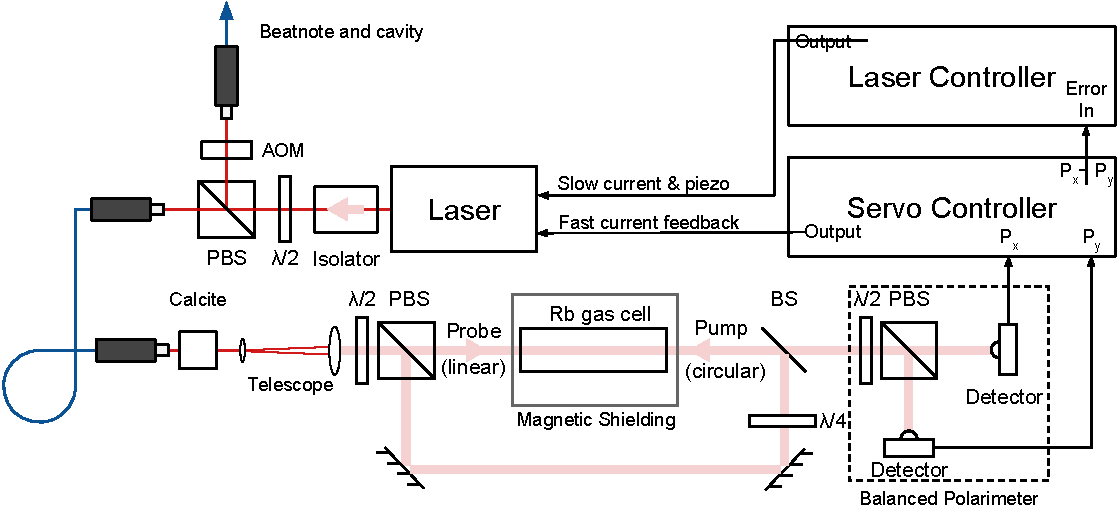
\includegraphics[width=\linewidth]{part1/Figs/fig1.pdf}
\caption{Schematic of a polarization spectroscopy (PS) apparatus.
The beam from the ECDL laser passes through an isolator before being split into two beams by a polarizing beam cube (PBS) and coupled into optical fibers.
One fibre leads to the PS setup and the other to other measurement or experimental apparatus.
The PS setup  consists of a polarization stabilizing calcite prism followed by a beam expanding telescope.
The expanded beam is then divided by a PBS into a linearly polarized probe and circularly polarized pump which counter-propagate, via a non-polarizing 50:50 beamsplitter (BS), through the magnetically shielded atomic gas sample.
The polarization rotation of the probe beam is then measured by a balanced polarimeter which consists of a $\lambda/2$ waveplate, PBS and two detectors.}
\label{polspec_schematic}
\end{figure}

The spectral profile of the difference in absorption coefficients for the circularly polarized components for the atomic medium in the vicinity of a resonance is a Lorentzian with width $\Gamma$, the inverse lifetime of the excited state of the resonant transition~\cite{demtroder_laser_2003}:
\begin{align}
\Delta \alpha = \frac{\Delta\alpha_0}{1+4\left(\frac{\delta}{\Gamma}\right)^2}.
\end{align}
Here $\delta=\omega_L-\omega_A$ is the detuning of the laser from the resonance, $\omega_L$ is the angular frequency of the laser and $\omega_A$ the angular frequency of the atomic resonance.
$\Delta\alpha_0$ is the difference in absorption coefficients for the $\sigma^\pm$ circular polarization components at zero detuning.

The refractive index and absorption of the medium are related through the Kramers-Kronig dispersion relation \cite{demtroder_laser_2003},
\begin{align}
\Delta n = \Delta\alpha_0 \frac{2c}{\omega_A \Gamma}\frac{\delta}{1+4\left(\frac{\delta}{\Gamma}\right)^2}.\label{result}
\end{align}
$\Delta\alpha_0$ is the sum over all $m_F$ ground states of the difference between absorption coefficients for each circular polarization, with $\delta=0$, weighted by the ground ($F, m_F$) and excited state ($F', m_{F\pm1}$) population differences,
\begin{align}
\Delta\alpha_0 = \sum_{m_F=-F}^{+F} \big[\alpha_{(F,m_F\rightarrow F',m_{F+1})}(P_{F,m_F}-P'_{F',m_{F+1}})\nonumber\\
-\alpha_{(F,m_F\rightarrow F',m_{F-1})}(P_{F,m_F}-P'_{F',m_{F-1}})\big].
\end{align}
The absorption coefficient for a given transition is $\alpha_{(F, m_F\rightarrow F',m_{F\pm1})}=N \sigma(\omega_L)$ where $N$ is the total number of interacting atoms, $\sigma(\omega_L)$ is the absorption cross section for the transition and $P_{F,m_F}$ refer to the populations of the various atomic states.

\subsection{Magnetic shielding}

\section{Fast Theory}

\subsection{from paper}
The atomic substate populations can be calculated using \glspl*{obe}~\cite{hughes_polarization_2009} but the standard steady-state solutions provide little insight into the behavior of the error signal when $\delta$ is changing faster than the evolution of the populations.
That evolution is limited to the spontaneous decay rate $\Gamma$, and hence for times $t\ll \tau=1/\Gamma$, the populations can be considered constant.
The \gls*{ps} signal is proportional to the refractive index difference given by Eq.~(\ref{result}), which describes a steep, background-free antisymmetric dispersive function, with bandwidth $1/t$ that can be much greater than $\Gamma$ (Fig.~\ref{sa_ps_spectra}).
Absorption-based frequency stabilization techniques such as \gls*{sa} rely on frequency-dependent changes to the atomic populations, rather than on the refractive index, resulting in dispersive signals over a much smaller capture range, with bandwidth limited to $\Gamma$.
SA is further limited if there are closely spaced hyperfine resonances or cross-over peaks.
Laser frequency noise can extend to frequencies much greater than $\Gamma$, where polarization spectroscopy still provides strong feedback and therefore can achieve much narrower laser linewidth.

\section{OBEs (timescale of state evolution, step in simulating)}

\section{Developments}

\subsection{Balanced Polarimeter}
When Wieman and H\"anch~\cite{wieman_doppler-free_1976} originally described \gls{ps} polarisation rotation was monitored with a nearly crossed polariser as shown in Figure \ref{figure:wieman_doppler-free_schematic}.
The polariser is crossed such that only a small proportion of the probe beam passes through them in the absence of the pump.
With the pump inducing anisotropy the rotation of the probe can be detected after the polarisers.

\begin{figure}
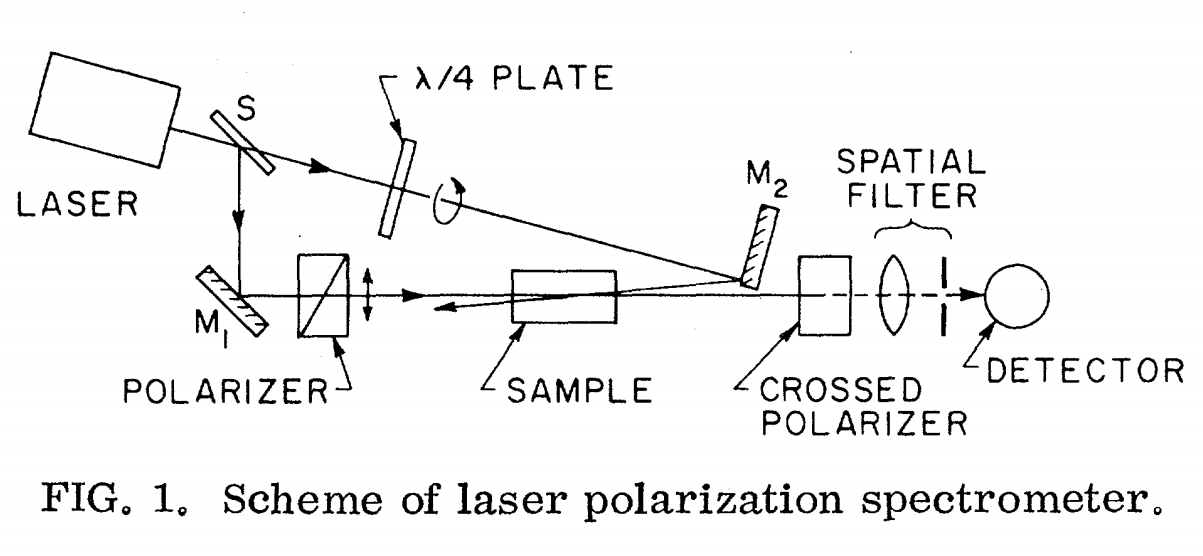
\includegraphics[width=\linewidth]{part1/Figs/wieman_doppler-free_schematic.png}
\caption{Figure stolen from Wieman and H\"anch paper.
Should probably redraw so I'm not plagiarizing.
Or ask how to cite it probably or some such.}
\label{figure:wieman_doppler-free_schematic}
\end{figure}

Pearson et al. proposed the alternative method of using a balanced polarimeter which provides a background-free signal with peak-to-peak height more than an order of magnitude greater than with the crossed polariser method~\cite{pearman_polarization_2002}.

\subsection{Beam splitter to co-propagate}

All papers thus far have ``snuck'' the pump beam through the vapour cell.

Figure with ``snucked'' and beam splitter configuration.

The angle of ``snucking'' has implications that there is math for...

Using a NBPS instead means you have an angle of 0.
The beam splitter has no effect on the polarisation as far as I can tell.

Pumped spectroscopy techniques such as \gls{ps} and \gls{sa}... spectral broadening due to angle stuff.

\subsection{High bandwidth feedback}


\subsection{Lincoln's magic detectors?}

\section{Experimental Setup (with details - fibres, calcite, etc.)}
\subsection{from paper - merge}
Two commercial Littrow configuration \glspl*{ecdl} were individually locked using \gls*{ps}.
The laser beam for each was split by a \gls*{pbs} and propagated through polarization-maintaining fibers to the \gls*{ps} locking system and linewidth measurements.
The locking beams were polarized with Glan-Thompson prisms (Fig.~\ref{polspec_schematic}) to eliminate residual polarization drift in the fibers.
Beam expanding telescopes were used to expand the beam to fill the apertures of the magnetic shielding, approximately \unit[1]{cm} diameter, allowing them to interact with more atoms to increase $|\Delta\alpha_0|$ and improve the \gls*{snr}.

The \gls*{pbs} balanced polarimeter error signal was generated with biased photodiodes (\unit[150]{MHz} bandwidth) and servo controllers (\unit[14]{MHz} bandwidth).
The servo controller integration zero-gain frequency was typically between \unit[100]{kHz} and \unit[1]{MHz}.
The diode modulation could be DC-coupled, with bandwidths of \unit[40]M{Hz} and \unit[10]{MHz}, or AC-coupled, \unit[100]{kHz}\,\textendash\,\unit[40]{MHz} and \unit[10]{kHz}\,\textendash\,\unit[10]{MHz}, depending on the laser.
The laser electronics provided control of the \glspl*{ecdl} piezoelectric transducer and diode injection current, with bandwidths of \unit[1]{kHz} and \unit[50]{kHz} respectively.


